\section{Struktur Aplikasi}
Didalam project Framework Phalcon, ada beberapa folder dan file penting dan menjadikan sebuah struktur aplikasi, berikut strukturnya sesuai dengan gambar ~\ref{fig:struktur}
\begin{figure}[h!]
\centerline{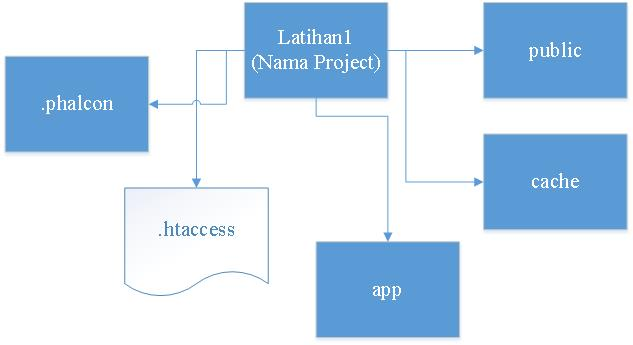
\includegraphics[width=0.8\textwidth]
{figures/struktur.JPG}}
\caption{Struktur yang ada didalam folder project Phalcon Framework}
\label{fig:struktur}
\end{figure}
Berikut penjelasan dari setiap struktur folder dan filenya:
\subsection{App}
folder ini berisikan script yang paling penting di project. Sebagai bagian terkomplit dari aplikasi web.
\subsubsection{Config}
folder \textit{config} berfungsi untuk membantu konfigurasi yang pasti dijalankan untuk menjalankan aplikasi secara lancar. Contohnya konfigurasi basis data, \textit{library}, dan \textit{services}.
\subsubsection{Controllers}
Berfungsi untuk memproses \textit{requests} dan menjalankan \textit{response} dari \textit{requests} tersebut.
\subsubsection{Library}
Berisikan \textit{library} dari luar \textit{library} bawaan Phalcon.
\subsubsection{Migrations}
Berisikan semua \textit{file} yang berhubungan dengan migrasi data. Dimana data tersebut juga bisa dipakai di framework lain.
\subsubsection{Models}
Berisikan logika-logika yang dibutuhkan untuk berinteraksi dengan basis data yang dipakai. Biasanya dipakai untuk representasi data.
\subsubsection{Views}
Di folder ini terdapat semua \textit{view} yang berhubungan dengan aplikasi web. Bisa dilihat oleh \textit{end-user} menggunakan bantuan dari \textit{Controller}
\subsection{Cache}
Direktori ini berfungsi untuk semua yang berhubungan dengan data yang memerlukan \textit{Caching}, yang mana akan membantu performa aplikasinya itu sendiri
\subsection{Public}
Disini termasuk semua folder yang berhubungan dengan manajemen aset seperti CSS, JavaScript, file hasil Upload, dan beberapa meta data
\subsection{File .htaccess}
Web Server yang berjalan di Apache Server memerlukan .htaccess sebagai file konfigurasi. Ketika ditempatkan di direktori nya, semua konfigurasi yang ditulis di file itu akan dijalankan selama server web nya mulai berjalan.